% Copyright 2004 by Till Tantau <tantau@users.sourceforge.net>.
%
% In principle, this file can be redistributed and/or modified under
% the terms of the GNU Public License, version 2.
%
% However, this file is supposed to be a template to be modified
% for your own needs. For this reason, if you use this file as a
% template and not specifically distribute it as part of a another
% package/program, I grant the extra permission to freely copy and
% modify this file as you see fit and even to delete this copyright
% notice. 

\documentclass{beamer}
\usepackage{graphicx}
\graphicspath{ {Images/} }
\usepackage{graphicx}

\usepackage{biblatex}

\addbibresource{ref.bib}

\usepackage{tikz}
\usetikzlibrary{shapes.geometric, arrows}
\tikzstyle{startstop} = [rectangle, rounded corners, minimum width=3cm, minimum height=1cm,text centered, draw=black, fill=red!30]
\tikzstyle{io} = [trapezium, trapezium left angle=70, trapezium right angle=110, minimum width=3cm, minimum height=1cm, text centered, draw=black, fill=blue!30]
\tikzstyle{process} = [rectangle, minimum width=3cm, minimum height=1cm, text centered, draw=black, fill=orange!30]
\tikzstyle{decision} = [diamond, minimum width=3cm, minimum height=1cm, text centered, draw=black, fill=green!30]
\tikzstyle{arrow} = [thick,->,>=stealth]
\tikzstyle{Memory} = [cylinder,shape border rotate=90,draw,minimum height=2.5cm,minimum width=2cm]

% There are many different themes available for Beamer. A comprehensive
% list with examples is given here:
% http://deic.uab.es/~iblanes/beamer_gallery/index_by_theme.html
% You can uncomment the themes below if you would like to use a different
% one:
%\usetheme{AnnArbor}
%\usetheme{Antibes}
%\usetheme{Bergen}
%\usetheme{Berkeley}
%\usetheme{Berlin}
%\usetheme{Boadilla}
%\usetheme{boxes}
%\usetheme{CambridgeUS}
%\usetheme{Copenhagen}
%\usetheme{Darmstadt}
%\usetheme{default}
%\usetheme{Frankfurt}
%\usetheme{Goettingen}
%\usetheme{Hannover}
%\usetheme{Ilmenau}
%\usetheme{JuanLesPins}
%\usetheme{Luebeck}
\usetheme{Madrid}
%\usetheme{Malmoe}
%\usetheme{Marburg}
%\usetheme{Montpellier}
%\usetheme{PaloAlto}
%\usetheme{Pittsburgh}
%\usetheme{Rochester}
%\usetheme{Singapore}
%\usetheme{Szeged}
%\usetheme{Warsaw}

\title{Automated Evaluation of Programming Assignments}

% A subtitle is optional and this may be deleted
%\subtitle{}

\author{Rishabh Manoj}
% - Give the names in the same order as the appear in the paper.
% - Use the \inst{?} command only if the authors have different
%   affiliation.

\institute{International Institute of Information Technology - Bangalore}

\date{\today}
% - Either use conference name or its abbreviation.
% - Not really informative to the audience, more for people (including
%   yourself) who are reading the slides online

\subject{Program Analysis}
% This is only inserted into the PDF information catalog. Can be left
% out. 

% If you have a file called "university-logo-filename.xxx", where xxx
% is a graphic format that can be processed by latex or pdflatex,
% resp., then you can add a logo as follows:

% \pgfdeclareimage[height=0.5cm]{university-logo}{university-logo-filename}
% \logo{\pgfuseimage{university-logo}}

% Delete this, if you do not want the table of contents to pop up at
% the beginning of each subsection:
\AtBeginSubsection[]
{
  \begin{frame}<beamer>{Outline}
    \tableofcontents[currentsection,currentsubsection]
  \end{frame}
}

% Let's get started
\begin{document}

\begin{frame}
  \titlepage
\end{frame}


% Section and subsections will appear in the presentation overview
% and table of contents.


\begin{frame}{Problem Statement}{}
    \begin{itemize}
        \item Automate the grading of programming solutions given a reference solution to a programming problem.\\
        \item Grades based on "correctness" measures of incorrect solutions.
    \end{itemize}
    
    
\end{frame}

\begin{frame}{Proposed Methods}{}
  \begin{itemize}
      \item \textbf{Gold Standard Solutions}: Separate given solns into \textit{correct} and \textit{incorrect} groups based on test-cases generated from reference solns. 
      \item \textbf{Similarity Measure}: Calculate the similarity measure of the correct solns with each other.
      \item \textbf{Clustering}: A fully connected graph can be constructed if each soln is considered as a node and the similarity measure value it's edge weight. Cluster this graph. Expected output is clusters of solutions with similar approaches.
      \item \textbf{Marking}: Calculate similarity measures of every incorrect solns to a representative solns of each of the clusters. Assign grades based on the "closeness" to cluster.  
  \end{itemize}
  
\end{frame}

\begin{frame}{Model Architecture}

\begin{center}

 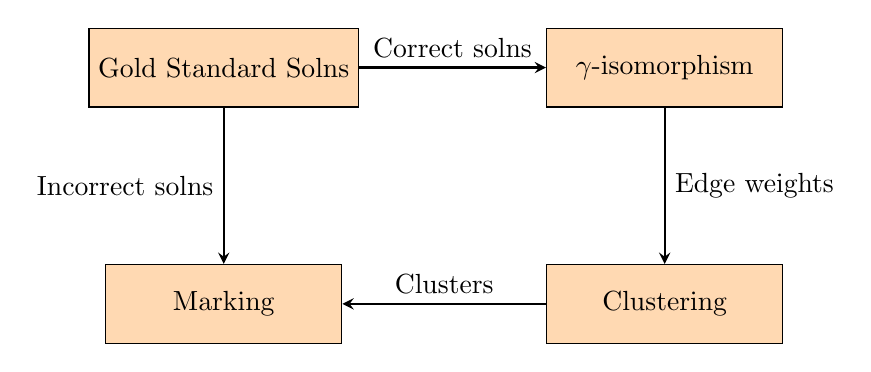
\begin{tikzpicture}[node distance=1.5cm]
   \node (pro1) [process] {Gold Standard Solns};
   \node (pro2) [process, right of=pro1, xshift = 4.1cm] {$\gamma$-isomorphism};
   \node (pro3) [process, below of=pro2, yshift = -1.5cm] {Clustering};
   \node (pro4) [process, left of=pro3, xshift = -4.1cm] {Marking};
   
   \draw [arrow] (pro1) -- node[anchor=south] {Correct solns} (pro2);
   \draw [arrow] (pro2) -- node[anchor=west] {Edge weights} (pro3);
   \draw [arrow] (pro3) -- node[anchor=south] {Clusters} (pro4);
    \draw [arrow] (pro1) -- node[anchor=east] {Incorrect solns} (pro4);
 \end{tikzpicture}    

\end{center}

\end{frame}

\begin{frame}{Similarity Measure}{Definitions}
    \begin{enumerate}
        \item \textbf{Data dependency:} A data dependency is a situation in which a program statement refers to the data of a preceding statement.\\
        \item \textbf{Control dependency:} Control dependency is a situation in which a program instruction executes if the previous instruction evaluates in a way that allows its execution. (\textit{if} statements, \textit{while} $\cdots$)\\
        \item \textbf{Isomorphism:} A graph can exist in different forms having the same number of vertices,edges and
also having same edge connectivity. Such graphs are called isomorphic graphs.\\
    \end{enumerate}
    
\end{frame}

\begin{frame}{Similarity Measure}{Definitions}
    \textbf{Program Dependence Graph:}\\ Program dependence graph (PDG) is a graphical representation of the source code of a program. Basic statements, like variable declarations, assignments, and procedure calls, are represented by program vertices in PDG’s. The data and control
dependencies between statements are represented by edges between program vertices
in PDG’s.\\

\end{frame}

\begin{frame}{Similarity Measure}
\begin{itemize}
    \item[] \textbf{$\gamma$-isomorphism:}\cite{Liu:2006:GDS:1150402.1150522}\\ 
   The central idea is to generate \textit{Program Dependence Graphs} for the solutions and check for sub-graph isomorphism between any two PDG's.\\
   If it is sub-graph isomorphic then based on the number of vertices mapped we calculate similarity.\\
    
    \textit{\textbf{Algorithm:}}
    \begin{itemize}
    \item Generate PDG's of the solution.
    \item Use $\gamma$-isomorphism method to calculate similarity between PDG's of all correct solutions. 
    \begin{itemize}
        \item This $\gamma$-isomorphism method checks for sub-graph isomorphism between the PDG's and calculates similarity measure.  
    \end{itemize}
    
    \end{itemize} 
\end{itemize}
  

\end{frame}

\begin{frame}{References:}
    
\printbibliography

\end{frame}
\end{document}


